\documentclass[aspectratio=169]{beamer}
\usetheme{Boadilla}



\usepackage[utf8]{inputenc}       % Codificação de entrada
\usepackage[T1]{fontenc}          % Codificação de saída
\usepackage[portuguese]{babel}   % Idioma
\usepackage{XCharter}             % Fonte principal
\AtBeginDocument{\fontsize{12}{12}\selectfont}

%\usepackage{geometry}
%\geometry{papersize={210mm,150mm}}

\usepackage{color}
\usepackage{graphicx}
\usepackage{amsmath, amssymb, amsfonts}
\usepackage{bm}
\usepackage{booktabs}
\usepackage{multirow}
\usepackage{caption}
\usepackage{subfigure}
\usepackage{wrapfig}
\usepackage{multicol}
\usepackage{sidecap}
\usepackage{tikz}
\usepackage{listings}
\usepackage{siunitx}
\usepackage{pdfpages}
\usepackage{float}
\usepackage{hyperref}
\usepackage{academicons}
\usepackage{setspace}

\newcommand{\eng}[1]{\textsl{#1}}
\newcommand{\cod}[1]{\texttt{#1}}

%----------------------------------------------------------------------------------------
%	AUTHOR / TITLE INFORMATION
%----------------------------------------------------------------------------------------
\title[Minicurso FPGAs]{\huge Introdução ao VHDL} %note that the optional arg in '[]' are displayed in the left column throughout the complete presentation
% adapt accordingly
% e.g., M.Sc. Intermediate Thesis Report
% or     B.Sc. Intermediate Thesis Report


\author[Prof. Dr. Oscar Eduardo Anacona Mosquera]{Prof. Dr. Oscar Eduardo Anacona Mosquera \newline\newline 
\scriptsize{oscar.mosquera@ufmt.br}
}%note that the optional arg in '[]' are displayed in the left column throughout the complete presentation



\AtBeginSection[]
{
	\begin{frame}{Conteúdo}
		\tableofcontents[currentsection]
	\end{frame}
}



%----------------------------------------------------------------------------------------
%	DOCUMENT
%----------------------------------------------------------------------------------------
\begin{document}
%----------------------------------------------------------------------------------------
%	TITLE PAGE
%----------------------------------------------------------------------------------------
%DO NOT CHANGE THIS FIRST SLIDE 
\begin{frame}[plain]
\titlepage
%\vspace{3cm}
%\begin{center} \color{MULTurquoise} {Chair of Cyber-Physical-Systems}\end{center}

\end{frame}



%----------------------------------------------------------------------------------------
\section{Objetivos}
%----------------------------------------------------------------------------------------

\begin{frame}
	\frametitle{Objetivos}
	
	\begin{itemize}
		\justifying
		\item \textbf{Introdução à VHDL:}
		\begin{itemize}
			\justifying
			\item Compreender os fundamentos da VHDL como uma linguagem de descrição de hardware.
			%\item Explorar a evolução do fluxo de projeto em VHDL, desde suas origens até os métodos modernos.
		\end{itemize}
		
		\item \textbf{Modelo de um Arquivo VHDL: Composição e Estrutura:}
		\begin{itemize}
			\justifying
			\item Analisar a estrutura de um arquivo VHDL, incluindo entidades, arquiteturas e bibliotecas.
			%\item Compreender a composição de um modelo VHDL e sua importância no design de circuitos digitais.
		\end{itemize}
		
		\item \textbf{Declarações Concorrentes em VHDL:}
		\begin{itemize}
			\justifying
			\item Explorar declarações concorrentes em VHDL, como processos, blocos e sinais.
			%\item Compreender como as declarações concorrentes são usadas para descrever comportamentos simultâneos em circuitos digitais.
		\end{itemize}
		
		\item \textbf{Declarações Sequenciais em VHDL:}
		\begin{itemize}
			\justifying
			\item Analisar declarações sequenciais em VHDL, como o uso dos Flip-Flops.
			%\item Entender como as declarações sequenciais são usadas para descrever comportamentos que ocorrem em uma sequência específica.
		\end{itemize}
		
		\item \textbf{Máquinas de Estados Finitas em VHDL:}
		\begin{itemize}
			\justifying
			\item Compreender os princípios fundamentais das máquinas de estados finitas (FSMs).
			%\item Desenvolver habilidades para implementar FSMs em VHDL para sistemas sequenciais.
		\end{itemize}	
		
	\end{itemize}
\end{frame}




%
%
%
%
%
%
%%----------------------------------------------------------------------------------------
%\section{Introdução aos dispositivos e software de design da Altera}
%%----------------------------------------------------------------------------------------
%
%
%
%\begin{frame}{Classical digital design flow}
%	
%	
%	\begin{block}{Specifications}
%	\justifying
%	Projete um detetor de numeros primos para valores entre $0_{10}$ a $7_{10}$.O circuito deve ser capaz de indicar um número primo com um atraso inferior a 200 ns.
%	\end{block}	
%	
%	
%	\begin{block}{Functional design}
%	\justifying
%	A funcionalidade e o comportamento do sistema são definidos em termos de entradas, saídas e operações necessárias para realizar uma tarefa específica. 
%	\end{block}		
%	
%	\begin{figure}[h]
%		\centering
%		\includegraphics[width=0.57\textwidth]{Figs/fig86.png}
%	\end{figure}
%	
%\end{frame}
%%----------------------------------------------------------------------------------------
%
%
%\begin{frame}{Classical digital design flow}
%	
%	
%	\begin{block}{Synthesis}
%		\justifying
%		Processo de transformar uma descrição de alto nível do comportamento funcional de um sistema em uma representação física ou lógica que pode ser implementada em hardware.
%	\end{block}	
%	
%	\begin{figure}[h]
%	\centering
%	\includegraphics[width=0.57\textwidth]{Figs/fig87.png}
%	\end{figure}
%	
%	
%	\begin{block}{Technology mapping}
%		\justifying
%		Nesta fase, a \textbf{netlist} gerada durante a síntese lógica é mapeada para os recursos específicos disponíveis no hardware de destino.
%	\end{block}		
%	
%	\begin{figure}[h]
%		\centering
%		\includegraphics[width=0.57\textwidth]{Figs/fig88.png}
%	\end{figure}
%	
%\end{frame}
%%----------------------------------------------------------------------------------------
%
%\begin{frame}{Classical digital design flow}
%	
%	
%	\begin{block}{Place and route}
%		\justifying
%		Processo de transformar uma descrição de alto nível do comportamento funcional de um sistema em uma representação física ou lógica que pode ser implementada em hardware.
%	\end{block}	
%	
%	\begin{figure}[h]
%		\centering
%		\includegraphics[width=0.27\textwidth]{Figs/fig89.png}
%	\end{figure}
%	
%	
%	\begin{block}{Verification}
%		\justifying
%		Se concentra em garantir que o projeto atenda aos requisitos de funcionalidade, desempenho e confiabilidade estabelecidos durante a fase de especificação.
%	\end{block}		
%	
%	\begin{figure}[h]
%		\centering
%		\includegraphics[width=0.57\textwidth]{Figs/fig90.png}
%	\end{figure}
%	
%\end{frame}
%%----------------------------------------------------------------------------------------
%
%\begin{frame}{Classical digital design flow}
%	
%	
%	\begin{block}{Fabrication}
%		\justifying
%		O projeto em que o circuito integrado é efetivamente construído a partir do layout físico desenvolvido durante as etapas anteriores do projeto, como colocação e roteamento.
%	\end{block}	
%	
%	\begin{figure}[h]
%		\centering
%		\includegraphics[width=0.67\textwidth]{Figs/fig91.png}
%	\end{figure}
%	
%	
%	
%\end{frame}
%%----------------------------------------------------------------------------------------
%
%
%\begin{frame}{Portfólio completo de soluções da Altera}
%	
%	\begin{figure}[h]
%	\centering
%	\includegraphics[width=0.97\textwidth]{Figs/fig01.png}
%	\end{figure}
%	
%\end{frame}
%%----------------------------------------------------------------------------------------
%
%\begin{frame}{Software Quartus II}
%	
%	\begin{figure}[h]
%		\centering
%		\includegraphics[width=0.97\textwidth]{Figs/fig02.png}
%	\end{figure}
%	
%\end{frame}











%----------------------------------------------------------------------------------------
\section{Linguagem de descrição de hardware VHDL}
%----------------------------------------------------------------------------------------


\begin{frame}{VHDL}
	\justifying
	
	\begin{block}{}
		\justifying
		A VHDL permite que os engenheiros descrevam o comportamento e a estrutura de circuitos digitais complexos. Essa descrição pode incluir informações sobre sinais, portas, componentes, processos, temporização e outros aspectos do projeto.
	\end{block}
	
	\begin{itemize}
		\item \textbf{V}HSIC (Very High Speed Integrated Circuit)
		\item \textbf{H}ardware
		\item \textbf{D}escription
		\item \textbf{L}anguage
	\end{itemize}
	
\begin{alertblock}{}
``\textbf{Tell me how your circuit should behave and I will give you
hardware that does the job.}”
\end{alertblock}	
	
	
\end{frame}
%----------------------------------------------------------------------------------------

\begin{frame}{Principais características}
\justifying
	
	\begin{itemize}
		\justifying
		\item \textbf{Descrição de Hardware:} VHDL permite a descrição abstrata de sistemas digitais, abrangendo desde níveis mais altos de comportamento até detalhes de baixo nível.
		\item \textbf{Simulação e Verificação:} A linguagem é amplamente utilizada em simulação para verificar o comportamento e o desempenho dos projetos antes da implementação física.
		\item \textbf{Síntese Lógica:} VHDL é frequentemente utilizado em conjunto com ferramentas de síntese para transformar a descrição de alto nível em uma implementação específica em hardware.
		\item \textbf{Projeto de Circuitos Complexos:} É particularmente útil para projetar sistemas digitais complexos, como processadores, sistemas embarcados, e outros dispositivos eletrônicos.

	\end{itemize}
	
	
\end{frame}




\begin{frame}{Principais características}
	\justifying
	
	\begin{itemize}
		\justifying

		\item \textbf{Reutilização de Design:} A VHDL suporta a reutilização de design, permitindo que módulos e componentes sejam definidos e posteriormente utilizados em diferentes projetos
		\item \textbf{Padrão IEEE:} VHDL é um padrão IEEE (\textbf{Institute of Electrical and Electronics Engineers}), o que contribui para sua ampla aceitação e uso na indústria.
		\item \textbf{Síntese para FPGAs e ASICs:} Pode ser utilizado para a síntese de projetos em FPGAs ou ASICs, convertendo a descrição em hardware físico.
	\end{itemize}
	
	
\end{frame}









%----------------------------------------------------------------------------------------

\begin{frame}{Terminologia}
	\justifying
	
	\begin{itemize}
		\justifying
		\item \textbf{HDL:} uma limguagem de descrição de hardware é uma linguagem de programação de software usada para a modelagem de um circuito hardware.
		
		\item \textbf{Modelo comportamental:} um componente é descrito pela resposta das entradas e saídas.
		
		\item \textbf{Modelo estrutural:} um componente é descrito pela interconexão de componentes/primitivas de níveis mais baixos (\textbf{abordagem top-down design}).
		
		
	\end{itemize}
	
	
\end{frame}
%----------------------------------------------------------------------------------------

\begin{frame}{Modelo comportamental (Behavioral Modeling)}
	\justifying

	\begin{itemize}
	\justifying
	\item Somente a funcionalidade do circuito, não a estrutura.
	
	\item A descrição do hardware não está vinculada a uma implementação específica de hardware.

	
	
\end{itemize}

	
	\begin{figure}[h]
		\centering
		\includegraphics[width=0.67\textwidth]{Figs/fig03.png}
	\end{figure}
	
	
\end{frame}

%----------------------------------------------------------------------------------------

\begin{frame}{Modelo estrutural (Structural Modeling)}
	\justifying
	
	\begin{itemize}
		\justifying
		\item Funcionalidade e estrutura do circuito.
	\end{itemize}
	
	
	\begin{figure}[h]
		\centering
		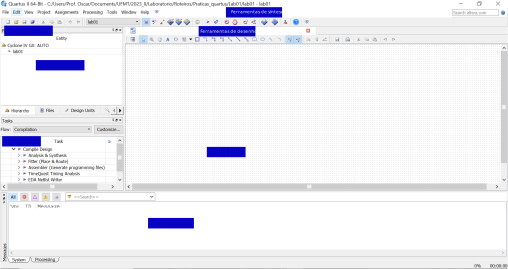
\includegraphics[width=0.67\textwidth]{Figs/fig04.png}
	\end{figure}
	
	
\end{frame}
%----------------------------------------------------------------------------------------
\begin{frame}{Terminologia}
	\justifying
	
	\begin{itemize}
		\justifying
		\item \textbf{Register Transfer Level (RTL):} um tipo de modelo comportamental, com o propósito de síntese. O hardware é implícito e é sintetizável.
		
		\item \textbf{Síntese:} traduzindo HDL para um circuito e, em seguida, otimizando o circuito representado.
		
		\item \textbf{Processo:} unidade básica de execução em VHDL (são convertidos para seu equivalente em hardware).
		
		
	\end{itemize}
	
	
\end{frame}
%----------------------------------------------------------------------------------------
\begin{frame}{RTL Synthesis}
	\justifying
	
	
	\begin{figure}[h]
		\centering
		\includegraphics[width=0.75\textwidth]{Figs/fig05.png}
	\end{figure}
	
	
\end{frame}
%----------------------------------------------------------------------------------------
\begin{frame}{Translation of VHDL Code into a Circuit}
	\justifying
	
	
	\begin{figure}[h]
		\centering
		\includegraphics[width=0.5\textwidth]{Figs/fig93.png}
	\end{figure}
	
	
\end{frame}



%----------------------------------------------------------------------------------------

%\begin{frame}{Typical PLD Design Flow}
%	\justifying
%	
%	
%	\begin{figure}[h]
%		\centering
%		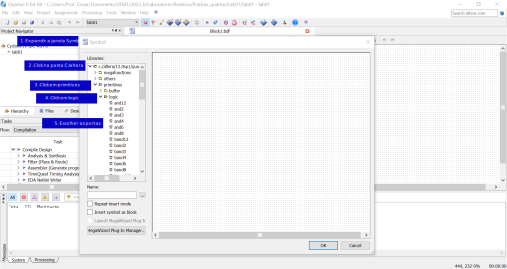
\includegraphics[width=0.97\textwidth]{Figs/fig06.png}
%	\end{figure}
%	
%	
%\end{frame}
%----------------------------------------------------------------------------------------
%\begin{frame}{Typical RTL Synthesis and RTL Simulation Flows}
%	\justifying
%	
%	
%	\begin{figure}[h]
%		\centering
%		\includegraphics[width=0.97\textwidth]{Figs/fig07.png}
%	\end{figure}
%	
%	
%\end{frame}
%----------------------------------------------------------------------------------------
%\begin{frame}{Modern Digital Design Flow}
%	\justifying
%	
%	
%	\begin{figure}[h]
%		\centering
%		\includegraphics[width=0.6\textwidth]{Figs/fig92.png}
%	\end{figure}
%	
%	
%\end{frame}









%----------------------------------------------------------------------------------------
\begin{frame}{VDHL básico}
	\justifying
	
	\begin{itemize}
		\justifying
		\item A linguagem VHDL é composta por palavras-chave reservadas.
		
		\item A linguagem, em sua maior parte, não é sensível a maiúsculas e minúsculas.
		
		\item As declarações VHDL são terminadas com um ponto e vírgula, ``;".
		
		\item VHDL é insensível a espaços em branco.
		
		\item \textbf{-- : Comentário de fim de linha (EOL)}; tudo a partir do símbolo até o EOL é comentado.
		
		\item \textbf{/* */} : Comentário delimitado; tudo entre os símbolos é comentado.
	\end{itemize}
	
	
\end{frame}
%----------------------------------------------------------------------------------------
\begin{frame}{Palavras chave}
	\justifying
	
	
	\begin{figure}[h]
		\centering
		\includegraphics[width=0.5\textwidth]{Figs/fig27.png}
	\end{figure}
	
	
\end{frame}





%----------------------------------------------------------------------------------------
\begin{frame}{Unidades de Design VHDL}
	\justifying
	
	\begin{itemize}
		\justifying
		\item \textbf{Entidades (Entities):} Entidades definem a interface do componente, especificando seus sinais de entrada e saída. Elas são como um contrato que descreve o comportamento externo do componente. As entidades não contêm lógica interna.
		
		\item \textbf{Arquiteturas (Architectures):} Arquiteturas definem a lógica interna de uma entidade. Elas descrevem como os sinais de entrada são manipulados para produzir os sinais de saída. Uma entidade pode ter várias arquiteturas, cada uma representando uma implementação diferente.
		
		\item \textbf{Pacotes (Packages):} Pacotes são usados para agrupar constantes, tipos de dados, subprogramas e outras declarações que podem ser compartilhadas entre várias entidades e arquiteturas. Eles são úteis para promover a reutilização e a organização do código.
		
		

	\end{itemize}
	
	
\end{frame}


\begin{frame}{Unidades de Design VHDL}
	\justifying
	
	\begin{itemize}
		\justifying

		
		\item \textbf{Configurações (Configurations):} Configurações são usadas para associar uma entidade a uma arquitetura específica ou a outras entidades. Elas permitem configurar a hierarquia do projeto e selecionar as implementações desejadas para cada componente.
		
		\item \textbf{Bibliotecas (Libraries):} Bibliotecas são coleções de unidades de design relacionadas, como entidades, arquiteturas e pacotes. Elas ajudam a organizar e gerenciar o código, permitindo a reutilização de unidades em diferentes projetos.
		
		
	\end{itemize}
	
	
\end{frame}




%----------------------------------------------------------------------------------------
\begin{frame}{Unidades de Design VHDL}
	\justifying
	
	
	\begin{figure}[h]
		\centering
		\includegraphics[width=0.7\textwidth]{Figs/fig10.png}
	\end{figure}
	
	
\end{frame}
%----------------------------------------------------------------------------------------
%\subsection{Entidade de projeto}
%----------------------------------------------------------------------------------------
\begin{frame}{Declaração da Entidade}
	\justifying
	
	
	\begin{figure}[h]
		\centering
		\includegraphics[width=1\textwidth]{Figs/fig09.png}
	\end{figure}
	
	
\end{frame}
%----------------------------------------------------------------------------------------
\begin{frame}{Declaração da Entidade}
	\justifying
	
	
	\begin{figure}[h]
		\centering
		\includegraphics[width=0.97\textwidth]{Figs/fig11.png}
	\end{figure}
	
	
\end{frame}
%----------------------------------------------------------------------------------------
%\begin{frame}{Declaração da Entidade}
%	\justifying
%	
%	
%	\begin{figure}[h]
%		\centering
%		\includegraphics[width=0.3\textwidth]{Figs/fig12.png}
%	\end{figure}
%	
%	\begin{figure}[h]
%	\centering
%	\includegraphics[width=0.97\textwidth]{Figs/fig13.png}
%	\end{figure}
%
%	
%\end{frame}
%----------------------------------------------------------------------------------------
\begin{frame}{Declaração da Entidade}
	\justifying
	
	Há quatro modos possíveis de uma porta, são eles:
	
	\begin{itemize}
		\item \textbf{IN:} porta de entrada.
		\item \textbf{OUT:} porta de saída, não pode ser referenciado internamente pela arquitetura.
		\item \textbf{BUFFER:} a porta opera unicamente no modo saída, pode ser referenciado internamente pela arquitetura.
		\item \textbf{INOUT:} caracteriza uma porta bidirecional onde uma informação pode ser apresentada ou amostrada.
	\end{itemize}
	
	
	
\end{frame}
%----------------------------------------------------------------------------------------
%\subsection{Corpo da arquitetura}
%----------------------------------------------------------------------------------------
\begin{frame}{Corpo da arquitetura}
	\justifying
	
	
	\begin{block}{}
	\justifying
	A ``ARCHITECTURE" em VHDL é usada para definir o comportamento ou a estrutura interna de um componente digital descrito na linguagem. 
	
	\begin{itemize}
	\item Descreve a funcionalidade.
	\item Declarações são executadas concorrentemente (processos).
	\item Podem ser colocadas várias arquiteturas.
	\item \textbf{Behavioral:} mostra como funciona.
	\item \textbf{RTL:} A descrição dos designs é feita em termos de registradores.
	\item \textbf{Hybrid:} mistura de ambos estilos.
	\end{itemize}	
	
	\end{block}	

	
	
\end{frame}



\begin{frame}{Corpo da arquitetura}
	\justifying
	
	
	
	\begin{figure}[h]
		\centering
		\includegraphics[width=0.97\textwidth]{Figs/fig14.png}
	\end{figure}
	
	
	
\end{frame}










%----------------------------------------------------------------------------------------

\begin{frame}{Corpo da arquitetura}
	\justifying
	
	
	\begin{figure}[h]
		\centering
		\includegraphics[width=0.97\textwidth]{Figs/fig29.png}
	\end{figure}
	
	
	
\end{frame}
%----------------------------------------------------------------------------------------
\begin{frame}{Corpo da arquitetura}
	\justifying
	
	
	\begin{figure}[h]
		\centering
		\includegraphics[width=0.97\textwidth]{Figs/fig15.png}
	\end{figure}
	
	
	
\end{frame}
%----------------------------------------------------------------------------------------






%----------------------------------------------------------------------------------------
\begin{frame}{VHDL- Estrutura Básica de Modelagem}
	\justifying
	
	
	\begin{figure}[h]
		\centering
		\includegraphics[width=0.77\textwidth]{Figs/fig16.png}
	\end{figure}
	
	
	
\end{frame}
%----------------------------------------------------------------------------------------
%\subsection{Classes de objetos}
%----------------------------------------------------------------------------------------
%\begin{frame}{Classes de objetos}
%	\justifying
%	
%	
%	\begin{itemize}
%	\item \textbf{CONSTANT:} valor estático.    
%	\item \textbf{SIGNAL:} 	sinais são objetos que podem ter o seu valor alterado, e são empregados em regiões de código concorrente e sequencial.
%	\item \textbf{FILE:} criação de arquivos.
%	\end{itemize}
%	
%	
%	Declaração de objetos das classes constante, variável e sinal:
%	
%	\begin{figure}[h]
%	\centering
%	\includegraphics[width=0.77\textwidth]{Figs/fig17.png}
%	\end{figure}
%	
%	
%	Exemplos de transferência de informação entre objetos:
%	
%	\begin{figure}[h]
%	\centering
%	\includegraphics[width=0.77\textwidth]{Figs/fig18.png}
%	\end{figure}	
%	
%\end{frame}
%----------------------------------------------------------------------------------------
%\begin{frame}{Classes de objetos}
%	\justifying
%	
%
%	
%	Exemplo de uma descrição completa:
%	
%	\begin{figure}[h]
%		\centering
%		\includegraphics[width=0.77\textwidth]{Figs/fig19.png}
%	\end{figure}
%	
%	
%	Representação esquemática do código:
%	
%	\begin{figure}[h]
%		\centering
%		\includegraphics[width=0.77\textwidth]{Figs/fig20.png}
%	\end{figure}	
%	
%\end{frame}
%----------------------------------------------------------------------------------------
%\begin{frame}{Classes de objetos}
%	\justifying
%	
%	
%	
%	\begin{block}{}
%	Sinais representam interconexões físicas (fios) que comunicam entre processos (funções).
%	\end{block}
%	
%	\begin{figure}[h]
%		\centering
%		\includegraphics[width=0.57\textwidth]{Figs/fig31.png}
%	\end{figure}
%	
%
%	
%\end{frame}










%----------------------------------------------------------------------------------------
%\subsection{Tipos de dados}
%----------------------------------------------------------------------------------------
\begin{frame}{Tipos de dados}
	\justifying
	

	
	\begin{figure}[h]
		\centering
		\includegraphics[width=0.97\textwidth]{Figs/fig21.png}
	\end{figure}
	
	
	
%	\begin{figure}[h]
%		\centering
%		\includegraphics[width=0.77\textwidth]{Figs/fig22.png}
%	\end{figure}	
	
\end{frame}

\begin{frame}{Tipos de dados}
	\justifying
	
	
	
%	\begin{figure}[h]
%		\centering
%		\includegraphics[width=0.97\textwidth]{Figs/fig21.png}
%	\end{figure}
	
	
	
	\begin{figure}[h]
		\centering
		\includegraphics[width=0.9\textwidth]{Figs/fig22.png}
	\end{figure}	
	
\end{frame}




%----------------------------------------------------------------------------------------
\begin{frame}{VHDL- pacotes std e IEEE}
	\justifying
	

	
	\begin{figure}[h]
		\centering
		\includegraphics[width=0.7\textwidth]{Figs/fig28.png}
	\end{figure}	
	
\end{frame}


%----------------------------------------------------------------------------------------
\begin{frame}{VHDL- pacotes std e IEEE: tipos sintetizáveis}
	\justifying
	
	
	
	\begin{figure}[h]
		\centering
		\includegraphics[width=0.65\textwidth]{Figs/fig36.png}
	\end{figure}	
	
\end{frame}








%----------------------------------------------------------------------------------------

\begin{frame}{VHDL- pacotes std e IEEE}
	\justifying
	
	\begin{block}{Type STD$\_$LOGIC}
		9 logic value system (‘U’, ‘X’, ‘0’, ‘1’, ‘Z’, ‘W’, ‘L’, ‘H’, ‘-’)
		
	\begin{itemize}
	\item \textbf{1:} Logic high    
	\item \textbf{0:} Logic low
	\item \textbf{X:} Unknown
	\item \textbf{Z:} (not ‘z’) Tri-state
	\item \textbf{-:} Don’t Care
	\item \textbf{U:} Undefined
	\item \textbf{H:} Weak logic high
	\item \textbf{L:} Weak logic low
	\item \textbf{W:} Weak unknown
	\end{itemize}		
		
		
	\end{block}
	
	
	
	

	
\end{frame}





%----------------------------------------------------------------------------------------
\begin{frame}{Conversão de tipos de dados}
	\justifying
	
	
	
	\begin{figure}[h]
		\centering
		\includegraphics[width=0.45\textwidth]{Figs/vhdl-type-conversions.png}
	\end{figure}	
	
\end{frame}



%----------------------------------------------------------------------------------------
\begin{frame}{Definição de novos tipos}
	\justifying
	
	\begin{block}{}
	\justifying
	A linguagem VHDL permite a criação de novos tipos enumerados, físicos e compostos.
	\end{block}		
	
	\begin{figure}[h]
		\centering
		\includegraphics[width=0.97\textwidth]{Figs/fig23.png}
	\end{figure}
	
%	\begin{block}{Subtype}
%	\justifying
%	Sintetizável se o tipo base é sintetizável.
%	\end{block}		
%	
%	\begin{figure}[h]
%		\centering
%		\includegraphics[width=0.57\textwidth]{Figs/fig73.png}
%	\end{figure}
	
\end{frame}


\begin{frame}{Definição de novos tipos}
	\justifying
%	
%	\begin{block}{}
%		\justifying
%		A linguagem VHDL permite a criação de novos tipos enumerados, físicos e compostos.
%	\end{block}		
%	
%	\begin{figure}[h]
%		\centering
%		\includegraphics[width=0.97\textwidth]{Figs/fig23.png}
%	\end{figure}
	
	\begin{block}{Subtype}
		\justifying
		Sintetizável se o tipo base é sintetizável.
	\end{block}		
	
	\begin{figure}[h]
		\centering
		\includegraphics[width=0.57\textwidth]{Figs/fig73.png}
	\end{figure}
	
\end{frame}







%----------------------------------------------------------------------------------------
%\subsection{Operadores}
%----------------------------------------------------------------------------------------

\begin{frame}{Operadores}
	\justifying
	
	\begin{block}{}
		\justifying
		Os operadores definidos são divididos em classes que estabelecem a precedência na execução das operações.
	\end{block}		
	
	\begin{figure}[h]
		\centering
		\includegraphics[width=0.9\textwidth]{Figs/fig24.png}
	\end{figure}
	
	
\end{frame}
%----------------------------------------------------------------------------------------
\begin{frame}{Operadores}
	\justifying
	
	
	\begin{figure}[h]
		\centering
		\includegraphics[width=0.9\textwidth]{Figs/fig25.png}
	\end{figure}
	
	
\end{frame}
%----------------------------------------------------------------------------------------
\begin{frame}{Operadores}
	\justifying
	
	
	\begin{figure}[h]
		\centering
		\includegraphics[width=0.9\textwidth]{Figs/fig26.png}
	\end{figure}
	
	
\end{frame}
%----------------------------------------------------------------------------------------
\begin{frame}{Operadores}
	\justifying
	
	
	\begin{figure}[h]
		\centering
		\includegraphics[width=0.77\textwidth]{Figs/fig30.png}
	\end{figure}
	
	
\end{frame}
%----------------------------------------------------------------------------------------
\begin{frame}{Operadores: sinais usadas como interligação}
	\justifying
	
	
	\begin{figure}[h]
		\centering
		\includegraphics[width=0.77\textwidth]{Figs/fig32.png}
	\end{figure}
	
	
\end{frame}
%----------------------------------------------------------------------------------------
\begin{frame}{Operadores: função aritmética}
	\justifying
	
	
	\begin{figure}[h]
		\centering
		\includegraphics[width=0.77\textwidth]{Figs/fig33.png}
	\end{figure}
	
	
\end{frame}
%----------------------------------------------------------------------------------------
%\subsection{Sobrecarga de Operadores}
%----------------------------------------------------------------------------------------
%\begin{frame}{Função/Pacote de Sobrecarga de Operadores}
%	\justifying
%	
%	Pacotes que definem funções de sobrecarga de operadores podem ser encontrados na BIBLIOTECA IEEE.
%	
%	\begin{itemize}
%	\item \textbf{STD$\_$LOGIC$\_$ARITH:} arithmetic functions   
%	\item \textbf{STD$\_$LOGIC$\_$SIGNED:} signed arithmetic functions
%	\item \textbf{STD$\_$LOGIC$\_$UNSIGNED:} unsigned arithmetic functions
%	\item \textbf{NUMERIC$\_$STD:} signed and unsigned arithmetic
%	\end{itemize}
%	
%	Por exemplo, o pacote \textbf{STD$\_$LOGIC$\_$UNSIGNED} define algumas das seguintes funções:
%	
%	\begin{figure}[h]
%	\centering
%	\includegraphics[width=0.77\textwidth]{Figs/fig34.png}
%	\end{figure}
%	
%\end{frame}
%----------------------------------------------------------------------------------------
%\begin{frame}{Função/Pacote de Sobrecarga de Operadores}
%	\justifying
%	
%	
%	\begin{figure}[h]
%		\centering
%		\includegraphics[width=0.77\textwidth]{Figs/fig35.png}
%	\end{figure}
%	
%	
%\end{frame}
%----------------------------------------------------------------------------------------
\begin{frame}{Exemplo}
	\justifying
	
	
	\begin{figure}[h]
		\centering
		\includegraphics[width=0.77\textwidth]{Figs/fig37.png}
	\end{figure}
	
	
\end{frame}
%----------------------------------------------------------------------------------------
\section{Declarações Concorrentes}
%----------------------------------------------------------------------------------------
\begin{frame}{Declarações Concorrentes}
	\justifying
	
	\begin{itemize}
		\item Declaração \textbf{when}
		\item Declaração \textbf{select}
		\item Declaração \textbf{generate}
		\item Declaração \textbf{Process}
	\end{itemize}
	
	
	\begin{block}{Declarações concorrentes}
	VHDL é inerentemente concorrente em vez de sequencial.	
		
	\end{block}
	
%	\begin{figure}[h]
%		\centering
%		\includegraphics[width=0.57\textwidth]{Figs/fig38.png}
%	\end{figure}
	
	
\end{frame}


\begin{frame}{Declarações Concorrentes}
	\justifying
	
%	\begin{itemize}
%		\item Declaração \textbf{when}
%		\item Declaração \textbf{select}
%		\item Declaração \textbf{generate}
%		\item Declaração \textbf{Process}
%	\end{itemize}
%	
%	
%	\begin{block}{Declarações concorrentes}
%		VHDL é inerentemente concorrente em vez de sequencial.	
%		
%	\end{block}
	
	\begin{figure}[h]
		\centering
		\includegraphics[width=0.57\textwidth]{Figs/fig38.png}
	\end{figure}
	
	
\end{frame}
%----------------------------------------------------------------------------------------
%\subsection{select}
%----------------------------------------------------------------------------------------
\begin{frame}{Declaração select}
	\justifying
	

	
	
	\begin{block}{}
		\begin{itemize}
		\item Todas as possíveis condições devem ser consideradas.
		\item \textbf{when others} avalia todas as outras condições possíveis que não são especificamente declaradas.
		\end{itemize}
		
	\end{block}
	
	\begin{figure}[h]
		\centering
		\includegraphics[width=0.57\textwidth]{Figs/fig39.png}
	\end{figure}
	
	
\end{frame}
%----------------------------------------------------------------------------------------
\begin{frame}{Declaração select}
	\justifying
	
	
	\begin{figure}[h]
		\centering
		\includegraphics[width=0.77\textwidth]{Figs/fig40.png}
	\end{figure}
	
	
\end{frame}
%----------------------------------------------------------------------------------------
\begin{frame}{Declaração select}
	\justifying
	
	
	\begin{figure}[h]
		\centering
		\includegraphics[width=0.77\textwidth]{Figs/fig41.png}
	\end{figure}
	
	
\end{frame}
%----------------------------------------------------------------------------------------
%\subsection{when}
%----------------------------------------------------------------------------------------
\begin{frame}{Declaração when}
	\justifying
	
	
	\begin{figure}[h]
		\centering
		\includegraphics[width=0.97\textwidth]{Figs/fig42.png}
	\end{figure}
	
	\begin{figure}[h]
	\centering
	\includegraphics[width=0.57\textwidth]{Figs/fig43.png}
	\end{figure}
	
\end{frame}
%----------------------------------------------------------------------------------------
\begin{frame}{Declaração when}
	\justifying
	
	
	\begin{figure}[h]
	\centering
	\includegraphics[width=0.47\textwidth]{Figs/fig44.png}
	\end{figure}
	
	
\end{frame}
%----------------------------------------------------------------------------------------
%\subsection{Instanciação de componentes}
%----------------------------------------------------------------------------------------
\begin{frame}{Instanciação de componentes}
	\justifying
	
	\begin{block}{}
	Refere-se ao processo de criar uma instância ou uma cópia de uma entidade (design ou componente) dentro de um design maior. Isso permite reutilizar funcionalidades já definidas em um novo contexto, evitando a necessidade de reescrever o código.
	
	\end{block}
	
%	\begin{figure}[h]
%		\centering
%		\includegraphics[width=0.67\textwidth]{Figs/fig45.png}
%	\end{figure}
%	
	
\end{frame}

\begin{frame}{Instanciação de componentes}
	\justifying
	
%	\begin{block}{}
%		Refere-se ao processo de criar uma instância ou uma cópia de uma entidade (design ou componente) dentro de um design maior. Isso permite reutilizar funcionalidades já definidas em um novo contexto, evitando a necessidade de reescrever o código.
%		
%	\end{block}
	
	\begin{figure}[h]
		\centering
		\includegraphics[width=0.77\textwidth]{Figs/fig45.png}
	\end{figure}
	
	
\end{frame}
%----------------------------------------------------------------------------------------

\begin{frame}{Instanciação de componentes}
	\justifying
	
	
	\begin{figure}[h]
	\centering
	\includegraphics[width=0.5\textwidth]{Figs/fig46.png}
	\end{figure}
	

%    \begin{columns}
%	
%	\column{0.45\textwidth}
%	\begin{figure}[h]
%	\centering
%	\includegraphics[width=0.47\textwidth]{Figs/fig47.png}
%	\end{figure}
%	
%	\column{0.45\textwidth}
%	\begin{figure}[h]
%	\centering
%	\includegraphics[width=0.97\textwidth]{Figs/fig48.png}
%	\end{figure}
%	\end{columns}

	
\end{frame}


\begin{frame}{Instanciação de componentes}
	\justifying
	
	
%	\begin{figure}[h]
%		\centering
%		\includegraphics[width=0.37\textwidth]{Figs/fig46.png}
%	\end{figure}
	
	
	\begin{columns}
		
		\column{0.45\textwidth}
		\begin{figure}[h]
			\centering
			\includegraphics[width=0.57\textwidth]{Figs/fig47.png}
		\end{figure}
		
		\column{0.45\textwidth}
		\begin{figure}[h]
			\centering
			\includegraphics[width=1.1\textwidth]{Figs/fig48.png}
		\end{figure}
	\end{columns}
	
	
\end{frame}


%----------------------------------------------------------------------------------
%\subsection{Declaração de processos}
%----------------------------------------------------------------------------------
\begin{frame}{Declaração de processos}
	\justifying
	
	
	\begin{block}{Process()}
	O VHDL usa um processo para modelar atribuições de sinal baseadas em um evento. Dentro de um processo em VHDL, as declarações são executadas sequencialmente. Isso significa que as instruções dentro do bloco de processo são executadas em ordem, uma após a outra, seguindo a ordem em que foram escritas no código.
	\end{block}
	
	
	\begin{block}{Sensitivity list}
	Uma lista de sensibilidade é um mecanismo para controlar quando um processo é acionado (ou iniciado). Uma lista de sensibilidade contém uma lista de sinais aos quais o processo é sensível. Se houver uma transição em qualquer um dos sinais da lista, o processo será acionado e as atribuições de sinal no processo serão feitas. 
	\end{block}	
	
	
%	\begin{columns}
%		
%		\column{0.45\textwidth}
%		\begin{figure}[h]
%		\centering
%		\includegraphics[width=0.97\textwidth]{Figs/fig49.png}
%		\end{figure}
%		
%		\column{0.45\textwidth}
%		\begin{figure}[h]
%			\centering
%			\includegraphics[width=0.57\textwidth]{Figs/fig50.png}
%		\end{figure}
%	\end{columns}
%	
	
\end{frame}

%\begin{frame}{Declaração de processos}
%	\justifying
%	
%	
%%	\begin{block}{Process()}
%%		O VHDL usa um processo para modelar atribuições de sinal baseadas em um evento. Dentro de um processo em VHDL, as declarações são executadas sequencialmente. Isso significa que as instruções dentro do bloco de processo são executadas em ordem, uma após a outra, seguindo a ordem em que foram escritas no código.
%%	\end{block}
%%	
%%	
%%	\begin{block}{Sensitivity list}
%%		Uma lista de sensibilidade é um mecanismo para controlar quando um processo é acionado (ou iniciado). Uma lista de sensibilidade contém uma lista de sinais aos quais o processo é sensível. Se houver uma transição em qualquer um dos sinais da lista, o processo será acionado e as atribuições de sinal no processo serão feitas. 
%%	\end{block}	
%	
%	
%	\begin{columns}
%		
%		\column{0.45\textwidth}
%		\begin{figure}[h]
%			\centering
%			\includegraphics[width=1.2\textwidth]{Figs/fig49.png}
%		\end{figure}
%		
%		\column{0.45\textwidth}
%		\begin{figure}[h]
%			\centering
%			\includegraphics[width=1.1\textwidth]{Figs/fig50.png}
%		\end{figure}
%	\end{columns}
%	
%	
%\end{frame}


%%----------------------------------------------------------------------------------------
\begin{frame}{Declaração de processos}
	\justifying
	
	\begin{figure}[h]
	\centering
	\includegraphics[width=0.67\textwidth]{Figs/fig51.png}
	\end{figure}
	
	
	
%	\begin{figure}[h]
%	\centering
%	\includegraphics[width=0.67\textwidth]{Figs/fig52.png}
%	\end{figure}	
%	
	
	
\end{frame}


\begin{frame}{Declaração de processos}
	\justifying
	
%	\begin{figure}[h]
%		\centering
%		\includegraphics[width=0.67\textwidth]{Figs/fig51.png}
%	\end{figure}
%	
	
	
	\begin{figure}[h]
		\centering
		\includegraphics[width=0.67\textwidth]{Figs/fig52.png}
	\end{figure}	
	
	
	
\end{frame}

%----------------------------------------------------------------------------------------

\begin{frame}{Declaração de processos}
	\justifying
	
	\begin{figure}[h]
		\centering
		\includegraphics[width=0.67\textwidth]{Figs/fig53.png}
	\end{figure}
	
	
	
	
\end{frame}
%%----------------------------------------------------------------------------------------
\begin{frame}{Declaração de processos}
	\justifying
	
	
	\begin{block}{Processos concorrentes}
	\begin{itemize}
		\item Uma arquitetura pode ter múltiplos processos concorrentes.
		\item Cada processo é executado em paralelo com outros processos. 
		\item Sim, a ordem das declarações dentro de um processo em VHDL importa significativamente. A ordem das declarações determina a sequência de operações executadas pelo processo e pode afetar o comportamento do circuito descrito pelo código VHDL.
	\end{itemize}
	
	\end{block}		
	
%	
%	\begin{figure}[h]
%		\centering
%		\includegraphics[width=0.47\textwidth]{Figs/fig54.png}
%	\end{figure}
%	
\end{frame}

\begin{frame}{Declaração de processos}
	\justifying
	
	
%	\begin{block}{Processos concorrentes}
%		\begin{itemize}
%			\item Uma arquitetura pode ter múltiplos processos concorrentes.
%			\item Cada processo é executado em paralelo com outros processos. 
%			\item Sim, a ordem das declarações dentro de um processo em VHDL importa significativamente. A ordem das declarações determina a sequência de operações executadas pelo processo e pode afetar o comportamento do circuito descrito pelo código VHDL.
%		\end{itemize}
%		
%	\end{block}		
	
	
	\begin{figure}[h]
		\centering
		\includegraphics[width=0.47\textwidth]{Figs/fig54.png}
	\end{figure}
	
\end{frame}
%%----------------------------------------------------------------------------------------
%\begin{frame}{Declaração de processos}
%	\justifying
%	
%	
%	\begin{figure}[h]
%		\centering
%		\includegraphics[width=0.67\textwidth]{Figs/fig55.png}
%	\end{figure}
%	
%\end{frame}
%%%----------------------------------------------------------------------------------------
%\begin{frame}{Declaração de processos}
%	\justifying
%	
%	
%	\begin{figure}[h]
%		\centering
%		\includegraphics[width=0.87\textwidth]{Figs/fig56.png}
%	\end{figure}
%	
%\end{frame}
%%----------------------------------------------------------------------------------------
\begin{frame}{Declaração de processos}
	\justifying
	
	
	\begin{figure}[h]
		\centering
		\includegraphics[width=0.77\textwidth]{Figs/fig57.png}
	\end{figure}
	
\end{frame}
%%----------------------------------------------------------------------------------------
%\begin{frame}{Declaração de processos}
%	\justifying
%	
%	
%	\begin{figure}[h]
%		\centering
%		\includegraphics[width=0.87\textwidth]{Figs/fig58.png}
%	\end{figure}
%	
%\end{frame}
%%----------------------------------------------------------------------------------------
\begin{frame}{Signals vs Variables}
	\justifying
	
	
	\begin{figure}[h]
		\centering
		\includegraphics[width=0.77\textwidth]{Figs/fig59.png}
	\end{figure}
	
\end{frame}
%%----------------------------------------------------------------------------------------
\section{Declarações sequenciais}
%%----------------------------------------------------------------------------------------
\begin{frame}{Declarações sequenciais}
	\justifying
	
	Declarações sequenciais devem estar dentro de processos.
	
	\begin{block}{}
	\begin{itemize}
		\item IF-THEN
		\item CASE 
		\item Looping statements
		\item WAIT
	\end{itemize}
	
	\end{block}		
	
	
	
\end{frame}
%%----------------------------------------------------------------------------------------
%\subsection{Declarações IF-THEN}
%%----------------------------------------------------------------------------------------
\begin{frame}{Declarações IF-THEN}
	\justifying
	
	\begin{figure}[h]
	\centering
	\includegraphics[width=0.87\textwidth]{Figs/fig60.png}
	\end{figure}
	
	
	
\end{frame}
%%----------------------------------------------------------------------------------------
\begin{frame}{Declarações IF-THEN}
	\justifying
	
	\begin{figure}[h]
		\centering
		\includegraphics[width=0.87\textwidth]{Figs/fig61.png}
	\end{figure}
	
	
	
\end{frame}
%%----------------------------------------------------------------------------------------
%\begin{frame}{Declarações IF-THEN}
%	\justifying
%	
%	\begin{figure}[h]
%		\centering
%		\includegraphics[width=0.87\textwidth]{Figs/fig64.png}
%	\end{figure}
%	
%	
%	\begin{figure}[h]
%	\centering
%	\includegraphics[width=0.87\textwidth]{Figs/fig65.png}
%	\end{figure}
%
%	
%\end{frame}
%%----------------------------------------------------------------------------------------
%\subsection{Declaração CASE}
%%----------------------------------------------------------------------------------------
\begin{frame}{Declaração CASE}
	\justifying
	
	
	\begin{block}{}
	\begin{itemize}
		\item Todas as condições são avaliadas ao mesmo tempo.
		\item Todas as possíveis condições devem ser consideradas. 
		\item \textbf{``WHEN OTHERS"} avalia todas as outras condições possíveis que não são especificamente declaradas.
	\end{itemize}
	
	\end{block}	
	
%	\begin{figure}[h]
%		\centering
%		\includegraphics[width=0.87\textwidth]{Figs/fig62.png}
%	\end{figure}
	
	
	
\end{frame}


\begin{frame}{Declaração CASE}
	\justifying
	
	
%	\begin{block}{}
%		\begin{itemize}
%			\item Todas as condições são avaliadas ao mesmo tempo.
%			\item Todas as possíveis condições devem ser consideradas. 
%			\item \textbf{``WHEN OTHERS"} avalia todas as outras condições possíveis que não são especificamente declaradas.
%		\end{itemize}
%		
%	\end{block}	
	
	\begin{figure}[h]
		\centering
		\includegraphics[width=0.87\textwidth]{Figs/fig62.png}
	\end{figure}
	
	
	
\end{frame}

%%----------------------------------------------------------------------------------------
%\begin{frame}{Declaração CASE}
%	\justifying
%	
%	
%	\begin{figure}[h]
%		\centering
%		\includegraphics[width=0.87\textwidth]{Figs/fig63.png}
%	\end{figure}
%	
%	
%	
%\end{frame}
%%----------------------------------------------------------------------------------------
%\begin{frame}{Declaração CASE}
%	\justifying
%	
%	\begin{figure}[h]
%		\centering
%		\includegraphics[width=0.57\textwidth]{Figs/fig66.png}
%	\end{figure}
%	
%	
%	\begin{figure}[h]
%		\centering
%		\includegraphics[width=0.57\textwidth]{Figs/fig67.png}
%	\end{figure}
%	
%	
%\end{frame}

%%----------------------------------------------------------------------------------------
%\subsection{Loop statements}
%%----------------------------------------------------------------------------------------
%\begin{frame}{Loop statements}
%	\justifying
%	
%	\begin{block}{}
%	\begin{itemize}
%		\item While loops
%		\item for loops
%	\end{itemize}
%	
%	\end{block}		
%	
%	
%	\begin{figure}[h]
%		\centering
%		\includegraphics[width=0.37\textwidth]{Figs/fig68.png}
%	\end{figure}
%	
%	
%	
%	
%\end{frame}
%%----------------------------------------------------------------------------------------
%\begin{frame}{Loop statements}
%	\justifying
%	
%	
%	\begin{figure}[h]
%		\centering
%		\includegraphics[width=0.87\textwidth]{Figs/fig69.png}
%	\end{figure}
%	
%	
%	
%	
%\end{frame}

%%----------------------------------------------------------------------------------------
%\subsection{Wait statements}
%%----------------------------------------------------------------------------------------
%\begin{frame}{Wait statements}
%	\justifying
%	
%	\begin{block}{}
%	\begin{itemize}
%	\item Pausa a execução do processo enquanto a declaração WAIT é satisfeita.
%	\item Tipos:
%		\begin{itemize}
%		\item WAIT ON $<$signal$>$
%		\item WAIT UNTIL $<$boolean expression$>$
%		\item WAIT FOR $<$time expression$>$
%		\item WAIT UNTIL (a='1') FOR 5 us
%		\end{itemize}	
%	\end{itemize}	
%	\end{block}	
%	
%	\begin{figure}[h]
%		\centering
%		\includegraphics[width=0.67\textwidth]{Figs/fig70.png}
%	\end{figure}
%	
%\end{frame}

%%----------------------------------------------------------------------------------------
%\subsection{Signal attributes}
%%----------------------------------------------------------------------------------------
%\begin{frame}{Signal attributes}
%	\justifying
%	
%	\begin{block}{}
%		Há situações em que desejamos descrever um comportamento que é baseado em mais do que apenas o valor atual de um sinal.
%	\end{block}	
%	
%	\begin{figure}[h]
%		\centering
%		\includegraphics[width=0.67\textwidth]{Figs/fig71.png}
%	\end{figure}
%	
%\end{frame}
%%----------------------------------------------------------------------------------------
%\begin{frame}{Signal attributes}
%	\justifying
%
%	
%	\begin{figure}[h]
%		\centering
%		\includegraphics[width=0.67\textwidth]{Figs/fig72.png}
%	\end{figure}
%	
%\end{frame}
%%----------------------------------------------------------------------------------------
\section{VHDL and Logic Synthesis}
%%----------------------------------------------------------------------------------------
\begin{frame}{VHDL and Logic Synthesis}
	\justifying
	
	
	\begin{figure}[h]
		\centering
		\includegraphics[width=0.87\textwidth]{Figs/fig74.png}
	\end{figure}
	
\end{frame}
%%----------------------------------------------------------------------------------------
\begin{frame}{VHDL and Logic Synthesis}
	\justifying
	
	
	\begin{figure}[h]
		\centering
		\includegraphics[width=0.87\textwidth]{Figs/fig75.png}
	\end{figure}
	
\end{frame}
%%----------------------------------------------------------------------------------------
\begin{frame}{VHDL and Logic Synthesis}
	\justifying
	
	
	\begin{figure}[h]
		\centering
		\includegraphics[width=0.77\textwidth]{Figs/fig76.png}
	\end{figure}
	
\end{frame}

%%----------------------------------------------------------------------------------------
\begin{frame}{VHDL and Logic Synthesis}
	\justifying
	
	
	\begin{figure}[h]
		\centering
		\includegraphics[width=0.77\textwidth]{Figs/fig76.png}
	\end{figure}
	
\end{frame}
%%----------------------------------------------------------------------------------------
\begin{frame}{VHDL and Logic Synthesis}
	\justifying
	
	Quantos registradores?
	
	\begin{figure}[h]
		\centering
		\includegraphics[width=0.32\textwidth]{Figs/fig77.png}
	\end{figure}
	
\end{frame}
%%----------------------------------------------------------------------------------------
\begin{frame}{VHDL and Logic Synthesis}
	\justifying
	
	
	\begin{figure}[h]
		\centering
		\includegraphics[width=0.87\textwidth]{Figs/fig78.png}
	\end{figure}
	
\end{frame}
%%----------------------------------------------------------------------------------------
%\begin{frame}{VHDL and Logic Synthesis}
%	\justifying
%	
%	Quantos registradores?
%	
%	\begin{figure}[h]
%		\centering
%		\includegraphics[width=0.87\textwidth]{Figs/fig79.png}
%	\end{figure}
%	
%\end{frame}
%%----------------------------------------------------------------------------------------
%\begin{frame}{VHDL and Logic Synthesis}
%	\justifying
%	
%	
%	\begin{figure}[h]
%		\centering
%		\includegraphics[width=0.47\textwidth]{Figs/fig80.png}
%	\end{figure}
%	
%\end{frame}
%%----------------------------------------------------------------------------------------
%\begin{frame}{VHDL and Logic Synthesis}
%	\justifying
%	
%	
%	\begin{figure}[h]
%		\centering
%		\includegraphics[width=0.87\textwidth]{Figs/fig81.png}
%	\end{figure}
%	
%\end{frame}
%%----------------------------------------------------------------------------------------
\section{Máquinas de Estados Finitas (FSMs)}
%%----------------------------------------------------------------------------------------
\begin{frame}{Máquinas de Estados Finitas (FSMs)}
	\justifying
	
	\begin{block}{}
	\begin{itemize}
		\item Utilizar um processo combinacional com uma declaração \textbf{CASE}.
		\item Utilizar atribuições de sinal condicionais e/ou selecionadas para cada saída.
	\end{itemize}	
	\end{block}	
	
	\begin{figure}[h]
		\centering
		\includegraphics[width=0.45\textwidth]{Figs/fig82.png}
	\end{figure}
	
\end{frame}

%%----------------------------------------------------------------------------------------
\begin{frame}{Máquinas de Estados Finitas (FSMs)}
	\justifying
	
	
	\begin{figure}[h]
		\centering
		\includegraphics[width=0.87\textwidth]{Figs/fig83.png}
	\end{figure}
	
\end{frame}
%%----------------------------------------------------------------------------------------
\begin{frame}{Máquinas de Estados Finitas (FSMs)}
	\justifying
	
	
	\begin{figure}[h]
		\centering
		\includegraphics[width=0.87\textwidth]{Figs/fig84.png}
	\end{figure}
	
\end{frame}
%%----------------------------------------------------------------------------------------
\begin{frame}{Máquinas de Estados Finitas (FSMs)}
	\justifying
	
	
	\begin{figure}[h]
		\centering
		\includegraphics[width=0.87\textwidth]{Figs/fig85.png}
	\end{figure}
	
\end{frame}
\section{Bibliografia}
%----------------------------------------------------------------------------------------
\begin{frame}{Bibliografia}
	\justifying
	
	\begin{itemize}
		\item Pedroni, V.A. Circuit Design with VHDL. MIT Press, 2004
		\item LaMeres, B. J. (2023). Introduction to Logic Circuits \& Logic Design with VHDL. Suíça: Springer International Publishing.

	\end{itemize}
	
\end{frame}


%

%\section{Software Quartus II Altera}
%%------



%\subsection{}
%
%\subsection{}
%
%\subsection{}
%
%\subsection{}
%
%\subsection{}
%
%\subsection{}
%
%%----------------------------------------------------------------------------------------
%\section{Ferramentas de depuração do projeto}
%%----------------------------------------------------------------------------------------
%
%\subsection{}
%
%\subsection{}
%
%\subsection{}
%
%\subsection{}
%
%\subsection{}
%
%\subsection{}
%
%
%
%
%%----------------------------------------------------------------------------------------
%\section{Simulação}
%%----------------------------------------------------------------------------------------
%
%\subsection{}
%
%\subsection{}
%
%\subsection{}
%
%\subsection{}
%
%\subsection{}
%
%\subsection{}
%
%
%
%
%%----------------------------------------------------------------------------------------
%\section{Utilização do kit FPGA}
%%----------------------------------------------------------------------------------------
%
%\subsection{}
%
%\subsection{}
%
%\subsection{}
%
%\subsection{}
%
%\subsection{}
%
%\subsection{}










%
%%----------------------------------------------------------------------------------------
%%	TOPIC AND MOTIVATION
%%----------------------------------------------------------------------------------------
%% NOTE that the topic and the motivation might be presented after   
%% the outlook, especially for presentations of more that 15 minutes! 
%\begin{frame}{Topic \& Motivation}
%% start the columns environment    
%\begin{columns} 
%% Column 1
%    \begin{column}{.4\textwidth}
%    
%    \begin{figure}[h] %or use htbp to place it inside the text blocks
%  	\centering
%  	\includegraphics[width=1.1\columnwidth]{pics/Franka_Panda_explosion-768x546.png}
%  	%\caption{\footnotesize{Illustration of a FRANKA Panda robot.}}
%  	\label{fig:panda}
%	\end{figure}
%    \end{column}
%% Column 2    
%    \begin{column}{.6\textwidth}
%        \begin{itemize}
%		\item[$\bullet$] Learning robot skills is challenging.
%		\item[$\bullet$] Humans learn skills in a few seconds.
%		\item[$\bullet$] Goal: Efficient learning algorithms \\ based on \textbf{my method}. 
%	\end{itemize}
%    \end{column}%
%    
%\end{columns}
% 
% 	Add a link to external sources if you want to show some videos, like \link{https://cps.unileoben.ac.at/wp/ICAR21_0108_VD_fi.mp4}{Video of our sensor glove}. 
%
%\end{frame}
%
%
%\section{Outlook}
%%----------------------------------------------------------------------------------------
%%	OUTLOOK
%%----------------------------------------------------------------------------------------
%\begin{frame}
%
%\frametitle[Outlook]{Outlook}
%\begin{itemize}
%	\item[$\bullet$] Topic \& Motivation.
%	\item[$\bullet$] Related Work.
%	\item[$\bullet$] Open Challenges.
%	\item[$\bullet$] Conceptual Overview of My Approach. 
%	\item[$\bullet$] Details to My Approach.
%	\item[$\bullet$] Evaluation Strategie \& Results.
%	\item[$\bullet$] Summary \& Future Work.
%\end{itemize}
%
%\end{frame}
%
%\section{Related Work}
%%----------------------------------------------------------------------------------------
%%	RELATED WORK
%%----------------------------------------------------------------------------------------
%\subsection{Related Work on Planning}
%
%\begin{frame}{Related Work on Planning}
%% start the columns environment    
%
%\begin{itemize}
%\item Paper XYZ implements ...
%\end{itemize}
%
%\end{frame}
%%----------------------------------------------------------------------------------------
%%	Sub Category of Related Work
%%----------------------------------------------------------------------------------------
%\subsection{Related Work on Reinforcement Learning}
%
%\begin{frame}{Related Work on Reinforcement Learning}
%% start the columns environment    
%
%\begin{itemize}
%\item Paper XYZ implements ...
%\end{itemize}
%
%\end{frame}
%
%
%\section{Method}
%%----------------------------------------------------------------------------------------
%%	METHOD DESCRIPTION
%%----------------------------------------------------------------------------------------
%% NOTE that the topic and the motivation might be presented prior to 
%% the outlook, especially for presentations of more than 15 minutes! 
%\subsection{Method Assumptions}
%
%\begin{frame}{My Method Assumptions}
%% start the columns environment    
%
%\begin{proof}
%The proposed method assumes xyz. Under this assumption it can be shown that $p(A) = p(A|B)$. 
%\end{proof}
%
%\end{frame}
%
%%----------------------------------------------------------------------------------------
%%	SUBSECTION on METHODS
%%----------------------------------------------------------------------------------------
%\subsection{Method Generalization}
%
%\begin{frame}{My Method Generalizability}
%% start the columns environment    
%
%\begin{block}{Generalizability}
%To demonstrate the generalizability of the method, an ablation study was evaluated.  
%\end{block}
%
%\begin{definition}
%In this work, we defined the initial parameters $\bm w$ to be zero. 
%\end{definition}
%
%\begin{example}
%More latex block definitions can be found at this \link{https://latex-beamer.com/tutorials/blocks/}{beamer tutorial page}.
%\end{example}
%
%\end{frame}
%
%%----------------------------------------------------------------------------------------
%%	SUBSECTION on METHODS
%%----------------------------------------------------------------------------------------
%\subsection{Method Extension}
%
%\begin{frame}{My Method Extension}
%% start the columns environment    
%
%Use  math environments to explain your method, e.g., 
%
% \begin{align}
%	A = 
%	\begin{bmatrix}
%		A_{11} & A_{21} \\
%		A_{21} & A_{22}
%	\end{bmatrix}
%\end{align}
%
%\begin{eqnarray}\label{eq:linRegModel}
%y &=& w_1 + w_2 x_1 + w_3 x_2 + \dots + w_{D+1} x_D, \nonumber \\
%y &=&  \bm x^T \bm w.
%\end{eqnarray}
%
%\end{frame}
%
%\begin{frame}{Method Details Animated}
%
%	%\textbf{Remember, a Multivariate Gaussian Distribution (MGD) is defined as:}
%	\vspace{.5cm}
%
%	\begin{overlayarea}{\textwidth}{\textheight}
%	\begin{itemize}
%		\item<2->For vectors $\bm x \in \sR^{Dx1}$, the Gaussian distribution is defined as 
%	\begin{eqnarray}\label{eq:GaussDist}
%		\N(\bm x | \bm \mu, \bm \Sigma) := \frac{1}{(2 \pi)^{D/2} {|\Sigma|}^{1/2}} \exp^{\{ -\frac{1}{2} \; (\bm x - \bm \mu)^T \; \bm 		\Sigma^{-1} \;   (\bm x - \bm \mu)  \}},
%	\end{eqnarray}
%	where $|\Sigma|$ denotes the \textit{determinant} of the \textit{covariance matrix} $\bm \Sigma \in \sR^{DxD}$.
%		\item<3->[]
%			\begin{block}{}
%				\textbf{The MGD is \textit{closed} under conditioning and marginalization.} This property implies that the 					resulting distributions, after applying these operations are also \textbf{Gaussian}!
%			\end{block}
%		\item<4->
%			$\rightarrow$ This is one of the main reasons why Gaussians are mathematically so appealing. 
%	\end{itemize}
%	\end{overlayarea}
%\end{frame}
%
%
%\section{Results}
%%----------------------------------------------------------------------------------------
%%	RESULTS DESCRIPTION
%%----------------------------------------------------------------------------------------
%\subsection{Evaluation Strategy}
%
%\begin{frame}{Evaluation Strategie}
%% start the columns environment    
%\textbf{Do not list more than five or six items per frame}\vspace{0.5cm}
%\begin{itemize}
%\item[$\circ$] Use single letters for scalars, i.e., $a \in \sR^1$.  
%\item[$\circ$] Vectors are written in bold, i.e., $\bm w \in \sR^{10}$.
%\item[$\circ$] Matrices are written in bold capital letters, i.e., $\bm M \in \sR^{\{10\;\times\;10\}}$. 
%\item[$\circ$] Use subscripts to denote elements in vectors, i.e., $w_i$ is part of $\bm w = [w_1, w_2, \dots, w_i]$.
%\item[$\circ$] Denote functions by single lower case letters, i.e., $x = f(y)$ which implements the transformation $f(y): \sR^1 \rightarrow \sR^1$.
%\end{itemize}
%
%\end{frame}
%
%%----------------------------------------------------------------------------------------
%%	RESULTS DESCRIPTION
%%----------------------------------------------------------------------------------------
%\subsection{Evaluation Strategy}
%
%\begin{frame}{Results \& Statistics}
%% start the columns environment    
%
%Use tables to present your results. Make sure to always list mean, standard deviation values and the number of runs.
%
%\vspace{1cm}
%\begin{table}[h]
%         \label{tab:exampleTableOne}
%	%\caption{Example table}
%	\centering
%	\begin{tabular}{llr}
%		\toprule
%		\multicolumn{2}{c}{Name} \\
%		\cmidrule(r){1-2}
%		First Name & Last Name & Grade \\
%		\midrule
%		John & Doe & $7.5$ \\
%		Richard & Miles & $5$ \\
%		\bottomrule
%	\end{tabular}
%\end{table}
%
%\end{frame}
%
%
%\begin{frame}{Video of the Results}
%% start the columns environment    
%
%\begin{center}
%        \embedvideo{\includegraphics[width=.7\textwidth]{pics/Franka_Panda_explosion-768x546.png}}{pics/sample-mp4-file-small.mp4}
%\end{center}
%
%\end{frame}
%
%
%\section{Summary \& Future Work}
%
%\subsection{Summary}
%%----------------------------------------------------------------------------------------
%%	SUMMARY
%%----------------------------------------------------------------------------------------
%\begin{frame}{Topic \& Motivation}
%% start the columns environment    
%\begin{columns} 
%% Column 1
%    \begin{column}{.4\textwidth}
%    
%    \begin{figure}[h] %or use htbp to place it inside the text blocks
%  	\centering
%  	\includegraphics[width=1.1\columnwidth]{pics/Franka_Panda_explosion-768x546.png}
%  	%\caption{\footnotesize{Illustration of a FRANKA Panda robot.}}
%  	\label{fig:panda}
%	\end{figure}
%    \end{column}
%% Column 2    
%    \begin{column}{.6\textwidth}
%        \begin{itemize}
%		\item[$\bullet$] Learning robot skills is challenging.
%		\item[$\bullet$] Humans learn skills in a few seconds.
%		\item[$\bullet$] Goal: Efficient learning algorithms \\ based on \textbf{my method}. 
%	\end{itemize}
%    \end{column}%
%    
%\end{columns}
% 
% 	Add a link to external sources if you want to show some videos, like \link{https://cps.unileoben.ac.at/wp/ICAR21_0108_VD_fi.mp4}{Video of our sensor glove}. 
%
%\end{frame}
%
%%----------------------------------------------------------------------------------------
%%	Discussion
%%----------------------------------------------------------------------------------------
%\subsection{Discussion}
%\begin{frame}{Discussion}
%% start the columns environment    
%\begin{block}{Assumptions}
%\begin{itemize}
%\item[$\bullet$] Data i.i.d.
%\item[$\bullet$] Model correlations are local and linear. 
%\item[$\bullet$] Number of modes has to be known.
%\end{itemize}
%\end{block}
%
%\begin{alertblock}{}
%However, many real-world applications can be modeled including robot manipulation tasks, locomotion and robot navigation.
%\end{alertblock}
%
%\end{frame}
%
%%----------------------------------------------------------------------------------------
%%	Future Work
%%----------------------------------------------------------------------------------------
%\subsection{Future Work}
%\begin{frame}{Evaluation Strategie}
%% start the columns environment    
%
%\begin{itemize}
%\item[$\bullet$] Use more complex evaluations. 
%\item[$\bullet$]  Use more complex models. 
%\item[$\bullet$]  Fix the assumption issue X.
%\end{itemize}
%
%\end{frame}
%
%
%%----------------------------------------------------------------------------------------
%%	THANK YOU 
%%----------------------------------------------------------------------------------------
%\begin{frame}[plain]
%\frametitle{Thank you for your attention!}
%% start the columns environment    
%\vfill
%\begin{columns} 
%% Column 1
%    \begin{column}{.8\textwidth}
%   	\begin{itemize}
%		\item \textbf{Joe Mann \& Hanna Ober} 
%		\item Chair of Cyber-Physical-Systems
%		\item Montanuniversität Leoben, Austria
%		\item \textbf{Email:}~\{joe.mann, hanna.ober\}@unileoben.ac.at
%		\item \textbf{Web:}~https://cps.unileoben.ac.at
%	\end{itemize}
%
%    \end{column}
%% Column 2    
%    \begin{column}{.2\textwidth}
%       
%    \end{column}%
%    
%\end{columns}
%
%\vfill 
%\scriptsize{
%\begin{block}{}
%\textbf{Disclaimer:} The lecture notes posted on this website are for personal use only. The material is intended for educational purposes only. Reproduction of the material for any purposes other than what is intended is prohibited. The content is to be used for educational and non-commercial purposes only and is not to be changed, altered, or used for any commercial endeavor without the express written permission of Professor Rueckert. 
%\end{block}
%}
%
%\vfill
%\begin{center} \color{MULTurquoise} {\scriptsize Template by Chair of Cyber-Physical-Systems, Univ.-Prof. Dr. Elmar Rueckert}\end{center}
%
%\end{frame}
%
%%----------------------------------------------------------------------------------------
%%	References
%%----------------------------------------------------------------------------------------
%\begin{frame}{References on Planning}
%% start the columns environment    
%
%\begin{itemize}
%\item[$\bullet$] [1] Paper by xyz... 
%\item[$\bullet$] [2] Paper by xyz... 
%\item[$\bullet$] [3] Paper by xyz... 
%\end{itemize}
%
%\end{frame}
%
%%----------------------------------------------------------------------------------------
%%	APPENDIX
%%----------------------------------------------------------------------------------------
%\section{APPENDIX}
%\begin{frame}{Details to my Method}
%% start the columns environment    
%
%\begin{itemize}
%\item[$\bullet$] Some details ...
%\item[$\bullet$] Some details ...
%\item[$\bullet$] Some details ... 
%\end{itemize}
%
%\end{frame}
%
%\begin{frame}{Details to my Results}
%% start the columns environment    
%
%\begin{itemize}
%\item[$\bullet$] Some details ...
%\item[$\bullet$] Some details ...
%\item[$\bullet$] Some details ... 
%\end{itemize}
%
%\end{frame}

\end{document}
